\section{Battery Models} \label{sec:kibam}
Part of the proposed solution is to ensure that battery level are maintain at an expectable level, in order to do this we need some way of modelling a battery, this section will go over three different battery models to determine what drawbacks there may be when using certain battery models. An important factor to consider when examining the battery models is the recovery effect, which can have large impact on the expected lifetime\cite{battery_model}. Recovery effect happen after a battery has been discharged for a period of time, the amount of current applied to the battery effects the recovery effect along with the battery capacity. The performance of the different models will be compared to the actual measured of a lithium-ion battery, measured are taken from \cite{battery_lifetime_analysis}, unfortunatly we are unable to obtain the specification for the lithium battery used in the paper as they are not listed in the paper. The measures for the different battery models is taken from \cite{battery_model} which also uses the same battery specification as the other paper they claim.

The Ideal model is very simplistic due to it only having two variables to determine the batteries lifetime(L), capacity(C) and load current(I). Capacity relates to the batteries amount of amp-hours, and load current is the constant discharge on the battery in amps. The formal for this is shown in \cref{eq:bm}.

\begin{equation}\label{eq:bm}
L=C/I
\end{equation}

Performance of the Ideal model can be seen in \cref{table:t-Ideal}. The table is divided into two parts, constant load and variable load, the column ``Meas, min'' show the actual measured readings of the lithium-ion battery under different loads. To the right the Ideal estimation are shown. In general the Ideal model overestimate the expected lifetime in all cases, shown in T1 the deviation from the actual measures differs by 28.58\%, a trend seems to appear in that lower amps often results in better predictions from the Ideal model with constant loads. Only T5 and T6 dose not apply to this, because T5 have a better prediction then T6 even though T5 has a higher load. During variable loads all cases overestimate by a substantial amount, the closest approximation is C5 during variable loads with a 18.5\% overestimation. The data shows that the Ideal model does a poor job of estimating the actual lifetime of a battery, which is properly because the Ideal model assumes linear effect for lifetime estimation. Additionally for variables loads the Ideal model does not consider recovery effect of the battery which further deviate results from the measured values. 

% Please add the following required packages to your document preamble:
% \usepackage[table,xcdraw]{xcolor}
% If you use beamer only pass "xcolor=table" option, i.e. \documentclass[xcolor=table]{beamer}
\begin{table}[H]
	\centering
	\scalebox{0.8}{
	\begin{tabular}{|llllll|lllll|}
		\hline
		\multicolumn{6}{|c|}{Constant load} & \multicolumn{5}{c|}{Variable load} \\ \hline
		\rowcolor[HTML]{EFEFEF} 
		\multicolumn{1}{|l|}{\cellcolor[HTML]{EFEFEF}Test} & \multicolumn{1}{l|}{\cellcolor[HTML]{EFEFEF}I, amps} & \multicolumn{1}{l|}{\cellcolor[HTML]{EFEFEF}Meas, min} & \multicolumn{1}{l|}{\cellcolor[HTML]{EFEFEF}Ideal, min} & \multicolumn{1}{l|}{\cellcolor[HTML]{EFEFEF}$\Delta$T} & \%$\Delta$ & \multicolumn{1}{l|}{\cellcolor[HTML]{EFEFEF}Test} & \multicolumn{1}{l|}{\cellcolor[HTML]{EFEFEF}Meas, min} & \multicolumn{1}{l|}{\cellcolor[HTML]{EFEFEF}Ideal, min} & \multicolumn{1}{l|}{\cellcolor[HTML]{EFEFEF}$\Delta$C} & \%$\Delta$ \\ \hline
		T1 & 222.7 & 141.0 & 181.3 & 40.3 & 28.58\% & C1 & 54.5 & 70.8 & 16.3 & 29.91\% \\ \hline
		\rowcolor[HTML]{EFEFEF} 
		T2 & 204.5 & 156.6 & 197.4 & 40.8 & 26.05\% & C2 & 73.3 & 91.9 & 18.6 & 25.38\% \\ \hline
		T3 & 108.3 & 307.8 & 372.8 & 65 & 21.12\% & C3 & 88.3 & 108.5 & 20.2 & 22.88\% \\ \hline
		\rowcolor[HTML]{EFEFEF} 
		T4 & 107.5 & 312.0 & 375.6 & 63.6 & 20.38\% & C4 & 136.0 & 163.0 & 27 & 19.85\% \\ \hline
		T5 & 94.9 & 358.2 & 425.4 & 67.2 & 18.76\% & C5 & 182.7 & 216.5 & 33.8 & 18.50\% \\ \hline
		\rowcolor[HTML]{EFEFEF} 
		T6 & 84.3 & 397.2 & 478.9 & 81.7 & 20.57\% & C6 & 59.0 & 74.7 & 15.7 & 26.61\% \\ \hline
		T7 & 75.5 & 448.2 & 534.8 & 86.6 & 19.32\% & C7 & 51.1 & 66.9 & 15.8 & 30.92\% \\ \hline
		\rowcolor[HTML]{EFEFEF} 
		T8 & 28.0 & 1248 & 1442 & 194 & 15.54\% & C8 & 55.0 & 70.8 & 15.8 & 28.73\% \\ \hline
		T9 & 19.5 & 1818 & 2071 & 253 & 13.92\% & C9 & 54.9 & 70.8 & 15.9 & 28.96\% \\ \hline
		\rowcolor[HTML]{EFEFEF} 
		T10 & 3.0 & 12690 & 13458 & 768 & 6.05\% & C10 & 142.7 & 171.3 & 28.6 & 20.04\% \\ \hline
	\end{tabular}}
	\caption{Comparison of Actual measure against Ideal model. Specification for the variable loads can be found in \cref{table:variable_loads_list}
	}
	\label{table:t-Ideal}
\end{table}

Peukert Model introduces a few new variables in comparison to the Ideal model, like the previous we still want to estimate the expected lifetime, but to better represent the battery a non-linear model is needed. Peukert fixes this by changing the formula to what is seen in \cref{eq:pm}. 

\begin{equation}\label{eq:pm}
L=(\frac{C}{I^k})
\end{equation}
\begin{itemize}
	\item L - lifetime in hours
	\item C - capacity in AH
	\item I - load current in amps
	\item k - Peukert Exponent
\end{itemize}

Unlike the previous model these parameter not as concrete. Acording to \cite{battery_modeling} C should be close to the value of the battery capacity and k should be between 1.2 and 1.7 to give the best results. This should be noted that this is only for constant loads. as it best illustrate how Peukert model functions\cite{battery_modeling}. k can sometimes be provided by the manufactors, since it can be hard to determine the exact value of k without actual testing a battery

\cref{table:t-Peukert} showcases the estimations using Peukert. In most cases Peukert overestimate except for one instance in test T10, it underestimate with 3.17\%. It seems to become more accurate the smaller the amps are, with the outlines, T5 and T6 Similarly to \cref{table:t-Ideal}. One thing to notices is that for variable loads it still has a high mismatch compared to measured values, this is due to Peukerts model not taken recovery effect into account. But overall Peukert performance better than the Ideal model.

\begin{table}[H]
	\centering
	\scalebox{0.8}{
	\begin{tabular}{|llllll|lllll|}
\hline
\multicolumn{6}{|c|}{Constant load} & \multicolumn{5}{c|}{Variable load} \\ \hline
\rowcolor[HTML]{EFEFEF} 
\multicolumn{1}{|l|}{\cellcolor[HTML]{EFEFEF}Test} & \multicolumn{1}{l|}{\cellcolor[HTML]{EFEFEF}I, amps} & \multicolumn{1}{l|}{\cellcolor[HTML]{EFEFEF}Meas, min} & \multicolumn{1}{l|}{\cellcolor[HTML]{EFEFEF}Peukert, min} & \multicolumn{1}{l|}{\cellcolor[HTML]{EFEFEF}$\Delta$T} & \%$\Delta$ & \multicolumn{1}{l|}{\cellcolor[HTML]{EFEFEF}Test} & \multicolumn{1}{l|}{\cellcolor[HTML]{EFEFEF}Meas, min} & \multicolumn{1}{l|}{\cellcolor[HTML]{EFEFEF}Peukert, min} & \multicolumn{1}{l|}{\cellcolor[HTML]{EFEFEF}$\Delta$C} & \%$\Delta$ \\ \hline
T1 & 222.7 & 141.0 & 154.5 & 13.5 & 9.57\% & C1 & 54.5 & 60.5 & 6 & 11.01\% \\ \hline
\rowcolor[HTML]{EFEFEF} 
T2 & 204.5 & 156.6 & 168.4 & 11.8 & 7.54\% & C2 & 73.3 & 79.1 & 5.8 & 7.91\% \\ \hline
T3 & 108.3 & 307.8 & 321.3 & 13.5 & 4.39\% & C3 & 88.3 & 93.8 & 5.5 & 6.23\% \\ \hline
\rowcolor[HTML]{EFEFEF} 
T4 & 107.5 & 312.0 & 323.7 & 11.7 & 3.75\% & C4 & 136.0 & 142.5 & 6.5 & 4.78\% \\ \hline
T5 & 94.9 & 358.2 & 367.5 & 9.3 & 2.60\% & C5 & 182.7 & 190.2 & 7.5 & 4.11\% \\ \hline
\rowcolor[HTML]{EFEFEF} 
T6 & 84.3 & 397.2 & 414.4 & 17.2 & 4.33\% & C6 & 59.0 & 64.4 & 5.4 & 9.15\% \\ \hline
T7 & 75.5 & 448.2 & 463.6 & 15.4 & 3.44\% & C7 & 51.1 & 56.5 & 5.4 & 10.57\% \\ \hline
\rowcolor[HTML]{EFEFEF} 
T8 & 28.0 & 1248 & 1270 & 22 & 1.76\% & C8 & 55.0 & 60.5 & 5.5 & 10.00\% \\ \hline
T9 & 19.5 & 1818 & 1835 & 17 & 0.94\% & C9 & 54.9 & 60.5 & 5.6 & 10.20\% \\ \hline
\rowcolor[HTML]{EFEFEF} 
T10 & 3.0 & 12690 & 12288 & -402 & -3.17\% & C10 & 142.7 & 148.8 & 6.1 & 4.27\% \\ \hline
\end{tabular}}
	\caption{Comparison of Actual measure against Peukert model. Specification for the variable loads can be found in \cref{variable_loads_list}
	}
	\label{table:t-Peukert}
\end{table}

\gls{kibam} uses two wells as an abstract concept to represent a battery. It consist of an available charge and a bound charge as shown in \cref{fig:kibam_wells}, c determines the ratio of the two wells based on the total capacity. Current can only be drawn from the available charge, when the available charges height $h_2$ is lower then bound charge height $h_1$, charge start to flow from bound charge to available charge until both wells are at equal height. The rate of this flow is determined by the value k, this simulate the recovery effect of the battery like previous models was not able to capture. To calculate $y{1}$ and $y{2}$ can be seen in \cref{eq:y1} and\cref{eq:y2} along with a short description of the variables used in these equations.

\begin{figure}[H]
	\center
	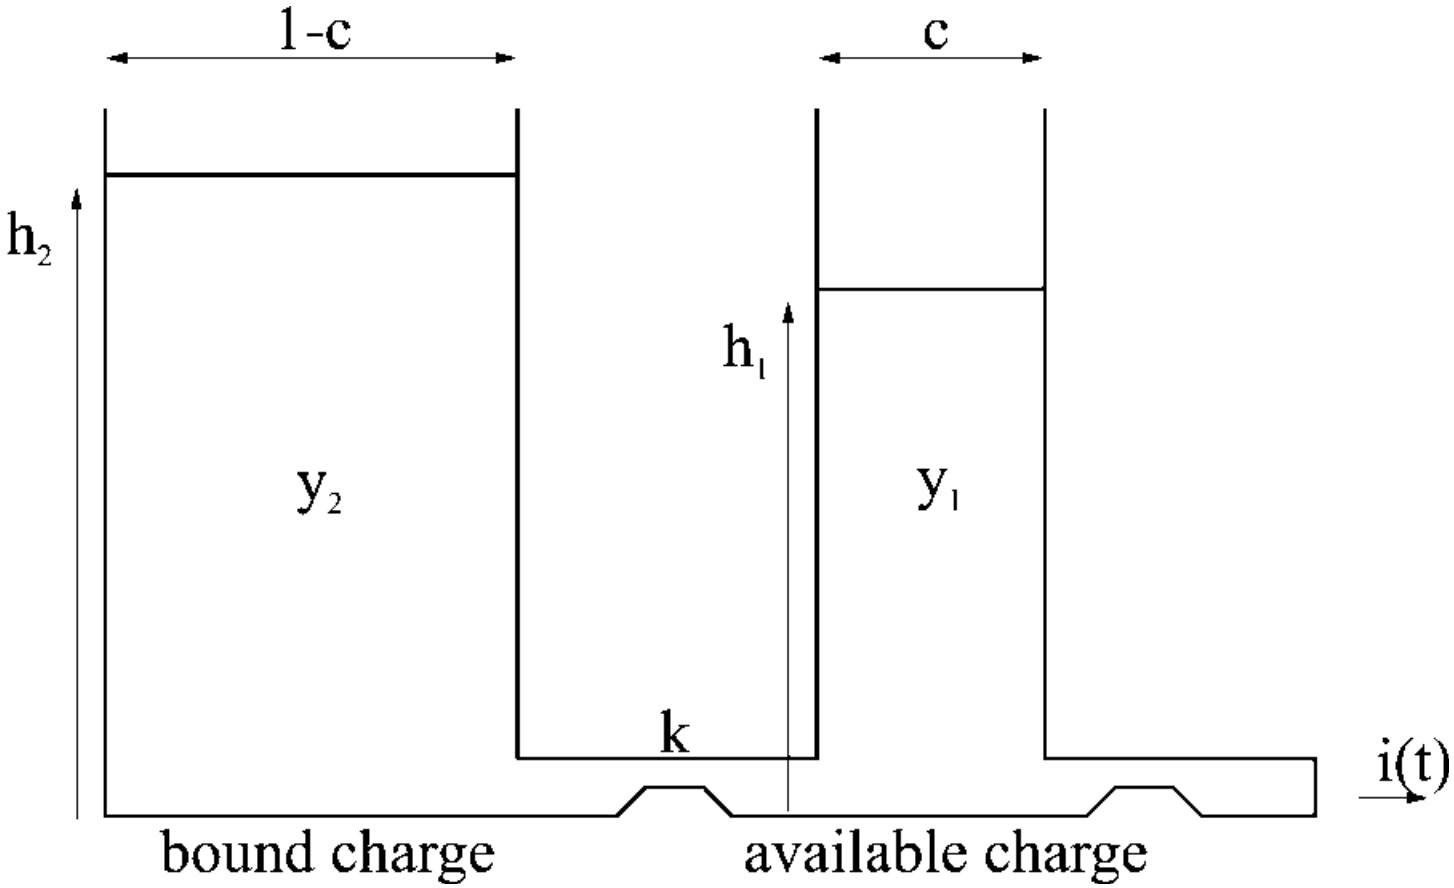
\includegraphics[width=\textwidth/2]{graphics/kibam.jpg}
	\caption{Displays the two wells of \gls{kibam}}
	\label{fig:kibam_wells}
\end{figure}

\begin{equation}\label{eq:y1}
y_1(t) = cCe^{-k't}+\frac{(y_0k'c-I)(1-e^{-k't})}{k'}-\frac{Ic(k't-1+e^{-k't})}{k'}
\end{equation}

\begin{equation}\label{eq:y2}
y_2(t) = (1-c)Ce^{-k't}+y_0(1-c)(1-e^{-k't})-\frac{I(1-c)(k't-1+e^{-k't})}{k'}
\end{equation}

C is capacity in Ah, e is Euler's number, k' is $k/c(1-c)$, k is a constant, t is time in hours, c is the ratio between available and bound charge, and I is the load current applied on the battery.

Performance of \gls{kibam} can be seen in \cref{table:t-KiBaM}. Under constant load the results vary, and he only indicating is that an amps above 110 and below 20 seems to give better results. Interesting for variable loads is that all of the predictions from \gls{kibam} underestimate compared to the measured values, some are fairly high though, like in case C7 it underestimate by 40.31\%.

\begin{table}[]
	\centering
	\scalebox{0.8}{
	\begin{tabular}{|l|lllll|llll|l|}
\hline
\multicolumn{6}{|c|}{Constant load} & \multicolumn{5}{c|}{Variable load} \\ \hline
\rowcolor[HTML]{EFEFEF} 
Test & \multicolumn{1}{l|}{\cellcolor[HTML]{EFEFEF}I, amps} & \multicolumn{1}{l|}{\cellcolor[HTML]{EFEFEF}Meas, min} & \multicolumn{1}{l|}{\cellcolor[HTML]{EFEFEF}KiBaM, min} & \multicolumn{1}{l|}{\cellcolor[HTML]{EFEFEF}$\Delta$T} & \%$\Delta$ & \multicolumn{1}{l|}{\cellcolor[HTML]{EFEFEF}Test} & \multicolumn{1}{l|}{\cellcolor[HTML]{EFEFEF}Meas, min} & \multicolumn{1}{l|}{\cellcolor[HTML]{EFEFEF}KiBaM, min} & $\Delta$T & \%$\Delta$ \\ \hline
T1 & 222.7 & 141.0 & 139.9 & -1.1 & -0.78\% & C1 & 54.5 & 36.3 & -18.2 & -33.39\% \\ \hline
\rowcolor[HTML]{EFEFEF} 
T2 & 204.5 & 156.6 & 156 & -0.6 & -0.38\% & C2 & 73.3 & 55.7 & -17.6 & -24.01\% \\ \hline
T3 & 108.3 & 307.8 & 331.4 & 23.6 & 7.67\% & C3 & 88.3 & 71.4 & -16.9 & -19.14\% \\ \hline
\rowcolor[HTML]{EFEFEF} 
T4 & 107.5 & 312.0 & 334.1 & 22.1 & 7.08\% & C4 & 136.0 & 123.6 & -12.4 & -9.12\% \\ \hline
T5 & 94.9 & 358.2 & 384 & 25.8 & 7.20\% & C5 & 182.7 & 175.7 & -7 & -3.83\% \\ \hline
\rowcolor[HTML]{EFEFEF} 
T6 & 84.3 & 397.2 & 437.5 & 40.3 & 10.15\% & C6 & 59.0 & 41.1 & -17.9 & -30.34\% \\ \hline
T7 & 75.5 & 448.2 & 493.3 & 45.1 & 10.06\% & C7 & 51.1 & 30.5 & -20.6 & -40.31\% \\ \hline
\rowcolor[HTML]{EFEFEF} 
T8 & 28.0 & 1248 & 1401 & 153 & 12.26\% & C8 & 55.0 & 38.1 & -16.9 & -30.73\% \\ \hline
T9 & 19.5 & 1818 & 2029 & 211 & 11.61\% & C9 & 54.9 & 34.8 & -20.1 & -36.61\% \\ \hline
\rowcolor[HTML]{EFEFEF} 
T10 & 3.0 & 12690 & 13417 & 727 & 5.73\% & C10 & 142.7 & 131.7 & -11 & -7.71\% \\ \hline
\end{tabular}}
	\caption{Comparison of Actual measure against \gls{kibam} model. Specification for the variable loads can be found in \cref{variable_loads_list}
	}
	\label{table:t-KiBaM}
\end{table}

Looking at all the results for the three battery models, it show that Peukerts model give overall better estimation for variable loads then Ideal and \gls{kibam}. But the advantage of using \gls{kibam} over Peukerts model under variable load is that \gls{kibam} seems always underestimate, which is good for our case, that ensure that we will never run into a case where the prediction cause the actual system to run out of energy. The Ideal is inferior to Peukerts and \gls{kibam} in almost all predictions, a summarize of the three different battery models can be found below.
\begin{itemize}
	\item Ideal model - linear representation of the battery with no support of recovery effect
	\item Peukert model - non-linear representation of the battery with no support of recovery effect
	\item \gls{kibam} - abstract representation of the battery with support of recovery effect
\end{itemize}
Since CORA can not use \gls{kibam} or Peukert model because \gls{cora} only support linearly priced automata and only natural numbers. The Ideal model will have to suffice.
